\pdfoutput=1
\documentclass[11pt]{article}

% Final version generation
% \usepackage[review]{acl}
\usepackage[]{acl}

\usepackage{graphicx}
\usepackage{caption}
\usepackage{subcaption}
\usepackage{tabularx}
\usepackage{array,multirow,graphicx}


% Standard package includes
\usepackage{times}
\usepackage{latexsym}
\usepackage{amsmath}
\usepackage{float}
\usepackage[shortlabels]{enumitem}

\usepackage[titletoc,toc,title]{appendix}

% Latin characters
\usepackage[T1]{fontenc}

% UTF8 Encoding 
\usepackage[utf8]{inputenc}

% Space saver
\usepackage{microtype}

% Alias for pcr police
\newcommand{\pol}[1]{{\fontfamily{pcr}\selectfont#1}}

\usepackage{cuted}

\title{SemEval-2020 Task 11: Experiments on a Novel Approach \\ for the Detection of Propaganda Techniques in News Articles\\
\vspace{0.2cm}
\small Natural Language Processing Project Paper, Fall 2021
}

\author{
Antoine Basseto,
Giacomo Camposampiero 
\and Andrea Pinto \\         
ETH Zurich - Swiss Federal Institute of Technology \\ 
\texttt{\{abasseto, gcamposampie, pintoa\}@ethz.ch}
}

\begin{document}
\maketitle

\begin{abstract}
This paper describes the design of our system contributing to the Task 11 of SemEval-2020 \cite{semeval} aiming to detect propaganda techniques in news articles.
We investigate a novel approach allowing the technique classification task (\pol{TC}) to work under relaxed assumptions and be more easily applicable to real-world scenarios, leading to changes in the span identification task (\pol{SI}) as well. Both models are built on top of heterogeneous pre-trained language models (\pol{PLMs}) such as \pol{BERT}, \pol{RoBERTa} and \pol{XLNet}.
The described architecture achieved an F$_1$-score of $0.46072$ on the \pol{SI} task (ranking $8/45$) and proved flawed for the \pol{TC} task, with important adjustments having to be made before being able to achieve an F$_1$-score of $0.57572$.
\end{abstract}

\section{Introduction}
The proliferation of online misinformation has led to a significant amount of research into the automatic detection of fake news \cite{fakenews}. However, most of the efforts have been concentrated on whole-document classification \cite{rashkin-etal-2017-truth} or analysis of the general patterns of online propaganda \cite{garimella2015, chatfield2015}, while little has been done so far in terms of fine-grained text analysis. This approach could complement existing techniques and allow the user to extract more informed and nuanced judgment on the piece being read. Moreover, it could also inform journalists on the pitfalls they might be falling into when writing articles.

In this context, Task 11 of SemEval-2020\footnote{The official task webpage: \url{https://propaganda.qcri.org/semeval2020-task11/}} \cite{semeval} aims to bridge this gap, facilitating the development of models capable of spotting text fragments where a defined set of propaganda techniques are being used. This shared task provides a well-annotated dataset of 536 news articles, which enables the participant to develop detection models that automatically spot a defined range of 14 propaganda techniques in written texts.

The focus of the task is broken down into two well-defined sub-tasks, namely (1) \textit{Span identification} \pol{(SI)} to detect the text fragments representative of a propaganda technique in the news articles and (2) \textit{Technique classification} \pol{(TC)} to detect the propaganda technique used in a given text span.

Our entire project is publicly available on our GitHub repository\footnote{\url{https://github.com/andreakiro/nlpropaganda}}. You can also see the results provided by our architecture on the leaderboard of the SemEval-2020 shared task, our team name being \textit{nlpboomers}.

\section{Related Work}
\subsection{Literature review}
Literature regarding fine-grained propaganda detection and analysis has known a significant development only in the last few years, mostly thanks to the different shared tasks that covered this particular topic \cite{da-san-martino-etal-2019-findings, finalsemeval}.

One of the first contributions can be traced back to \cite{da-san-martino-etal-2019-fine}, which proposed a \pol{BERT}-based model to detect propaganda spans and to classify their techniques.
In the NLP4IF-2019 shared task, the participants used pre-trained language models (\pol{PLM}s), LSTMs and ensembles to tackle the problem of fine-grained propaganda classification \cite{yoosuf-yang-2019-fine, vlad-etal-2019-sentence, tayyar-madabushi-etal-2019-cost}.
Also in SemEval-2020 most of the winning teams solutions relied on Transformers and ensembles \cite{aschern, morio-etal-2020-hitachi-semeval, dimov2020nopropaganda, jurkiewicz2020applicaai}.

Our work is especially related to the cited studies of winning teams of the SemEval-2020 shared-task. We decided to use the same \pol{PLM}s as the other teams, with the addition of \pol{XLNet}. However, we differ by tackling the \pol{TC} sub-task in a way none of the previous teams had explored, leading to other subtleties in the \pol{SI} sub-task as well.

\subsection{Pre-Trained Language Models (\pol{PLMs})}
In this study, three different types of Transformer-based \pol{PLM}s \cite{vaswani2017attention} were used to tackle the tasks. Note that during training, we also update the weight parameters of the pre-trained models in order to fine-tune them. \\
\textbf{\pol{BERT}} \cite{devlin2019bert} is the epoch-making Transformer-based masked language model. In our work, the \pol{BERT\textsubscript{BASE}} model was employed. \\
\textbf{\pol{RoBERTa}} \cite{roberta} is a fine-tuned \pol{BERT}-based model where the authors investigated hyperparameters and training data size. \pol{RoBERTa} has achieved state-of-the-art results. In our work, the \pol{RoBERTa\textsubscript{BASE}} model was employed. \\
\textbf{\pol{XLNet}} \cite{yang2020xlnet} is a state-of-the-art extended Transformer using an autoregressive method to learn bidirectional contexts by maximizing the expected likelihood over all permutations of the input sequence factorization order. In our work, the \pol{XLNet\textsubscript{LARGE}} model was employed.

\subsection{Technology stack}
We opted to implement our architecture in \pol{AllenNLP} \cite{allennlp}, a recent NLP research library developed by the Allen Institute for Artificial Intelligence. The framework is built on top of PyTorch \cite{NEURIPS2019_9015} and SpaCy \cite{spacy2}, and was explicitly designed for developing state-of-the-art deep learning models on a wide variety of NLP tasks. 

\section{Dataset}
\subsection{Data description}
The dataset used for the task, PTC-SemEval20 corpus \cite{semeval}, consists of a sample of news articles collected from mid-2017 to early 2019. The articles were retrieved from 13 propaganda and 36 non-propaganda news outlets, as labeled by Media Bias/Fact Check\footnote{https://mediabiasfactcheck.com}, and manually annotated by the organizers. The exact procedure of text labeling is discussed in depth in both \cite{da-san-martino-etal-2019-fine} and \cite{semeval}. 

The training and validation part of the corpus are the same as those presented in \cite{da-san-martino-etal-2019-fine}. The test part of the corpus consists of 90 additional news article in respect to the original evaluation articles, retrieved and annotated using the same procedure as the original. In total, the collection consists of 536 news articles containing 8,981 propaganda spans, that belong to one of the fourteen possible techniques.

\subsection{Data exploration}
Some statistics about the corpus (e.g. the number of instances and the average length in terms of tokens/characters for each propaganda technique, the average length of articles and others) were already given by the organizers as part of the shared task description paper \cite{semeval}.

One such piece of information provided by the organizers is the distribution of the different propaganda techniques in the datasets. Those results can be seen in Figure \ref{fig:tech_distr}, as reported in \cite{semeval}.

\begin{figure}[h]
    \centering
    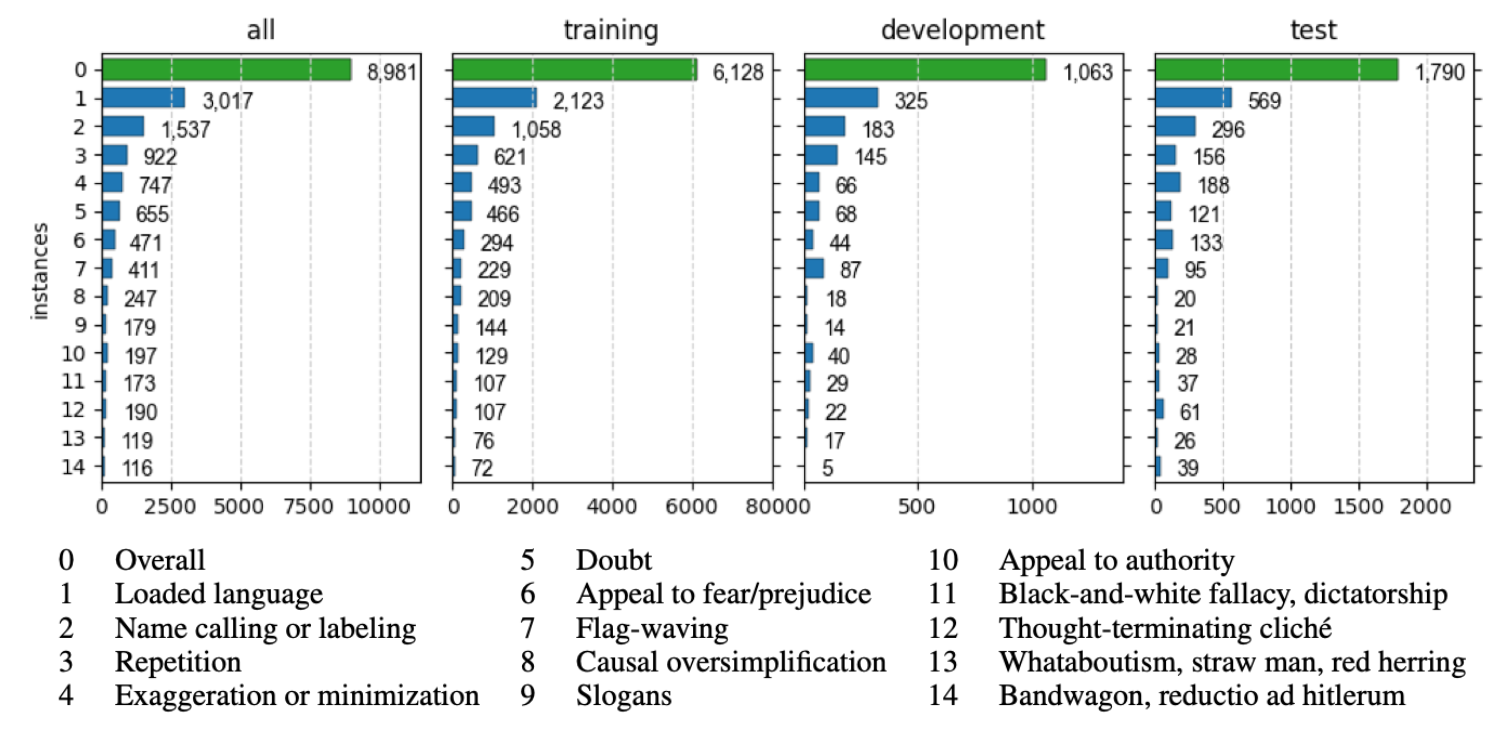
\includegraphics[width=0.5\textwidth]{images/technique_distr.png}
    \caption{Number of instances for each technique.}
    \label{fig:tech_distr}
\end{figure}

In addition to this data, a more fine-grained exploration of the training corpus was performed as one of the first steps in tackling the task. The main reasons for this additional exploration were:
\begin{itemize}
    \item To extract meaningful insights that could be used to infer robust and effective heuristics for span pruning in \pol{SI} preprocessing, as discussed in Section \ref{sec:si:preprocesing}.
    \item To justify some of our model architecture choices, especially for the \pol{SI} model and its specificities we discuss in Section \ref{sec:si}.
\end{itemize}

Some of the results of this analysis have been reported in Figures \ref{fig:nb-sentences} and \ref{fig:nb-tokens}. Due to space constraints, other results (e.g. the distribution over token categories in gold spans and border tokens), were omitted but can be accessed in our GitHub repository.

\begin{figure}[h]
    \centering
    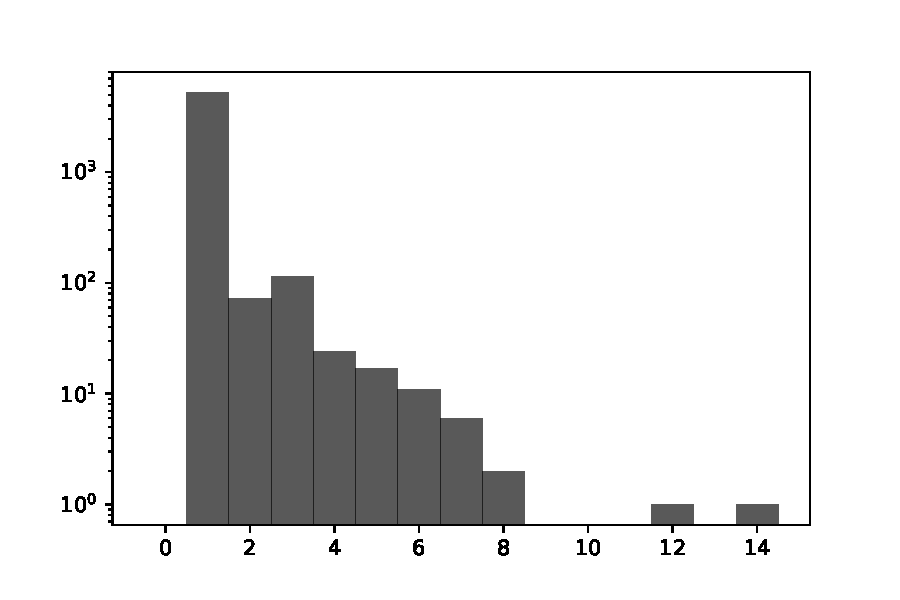
\includegraphics[width=0.4\textwidth]{images/sentences.pdf}
    \caption{Number of sentences in training gold spans.}
    \label{fig:nb-sentences}
\end{figure}

\begin{figure}[h]
    \centering
    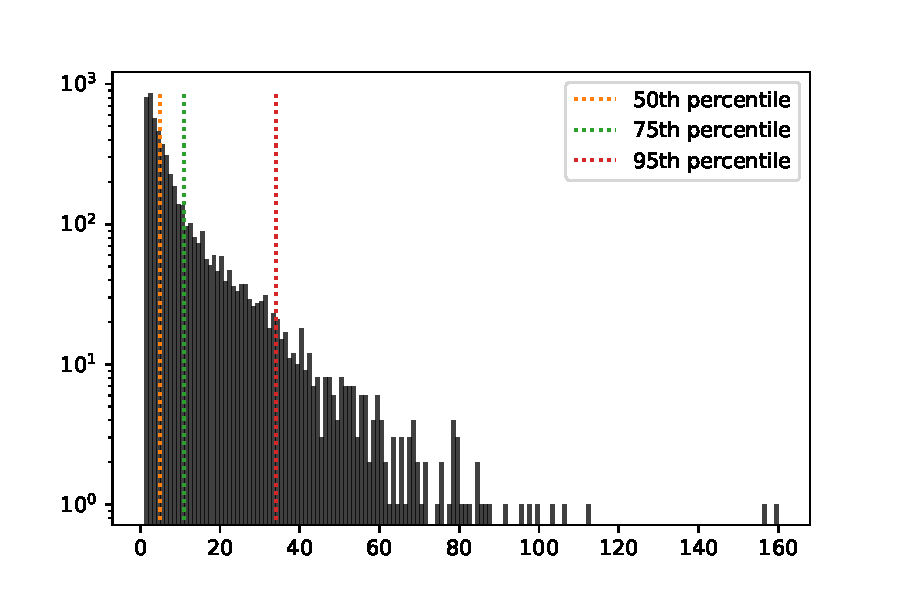
\includegraphics[width=0.4\textwidth]{images/tok_dist.pdf}
    \caption{Number of tokens in training gold spans.}
    \label{fig:nb-tokens}
\end{figure}

\section{System description} \label{sec:sys-desc}
Our approach was motivated by considering a real-world use of the \pol{TC} model. As described in the SemEval-2020 task, \pol{TC} models are supposed to classify a span as one of fourteen possible propaganda techniques, but this assumes that \pol{TC} models are always fed with spans that necessarily contain a propagandist argument. However, in a real-world scenario no such guarantees could be made, unless using a well-chosen list of manually selected spans.

\subsubsection*{Novel approach to architecture}
This conclusion resulted in two major changes compared to the architecture proposed in the SemEval-2020 shared task, that can be seen in Figure \ref{fig:general}, leading to an approach where the \pol{SI} model is part of the preprocessing stage of \pol{TC}:
\begin{enumerate}
    \item \pol{TC} model should train on the results provided by the \pol{SI} model, and not on a given set of gold spans already known to be propaganda.
    \item Because the \pol{SI} model will make mistakes, the \pol{TC} model should also be able to handle false positives and predict spans as "\textit{Not Propaganda}", adding an extra 15th class.
\end{enumerate}

\begin{figure*}[h]
    \centering
    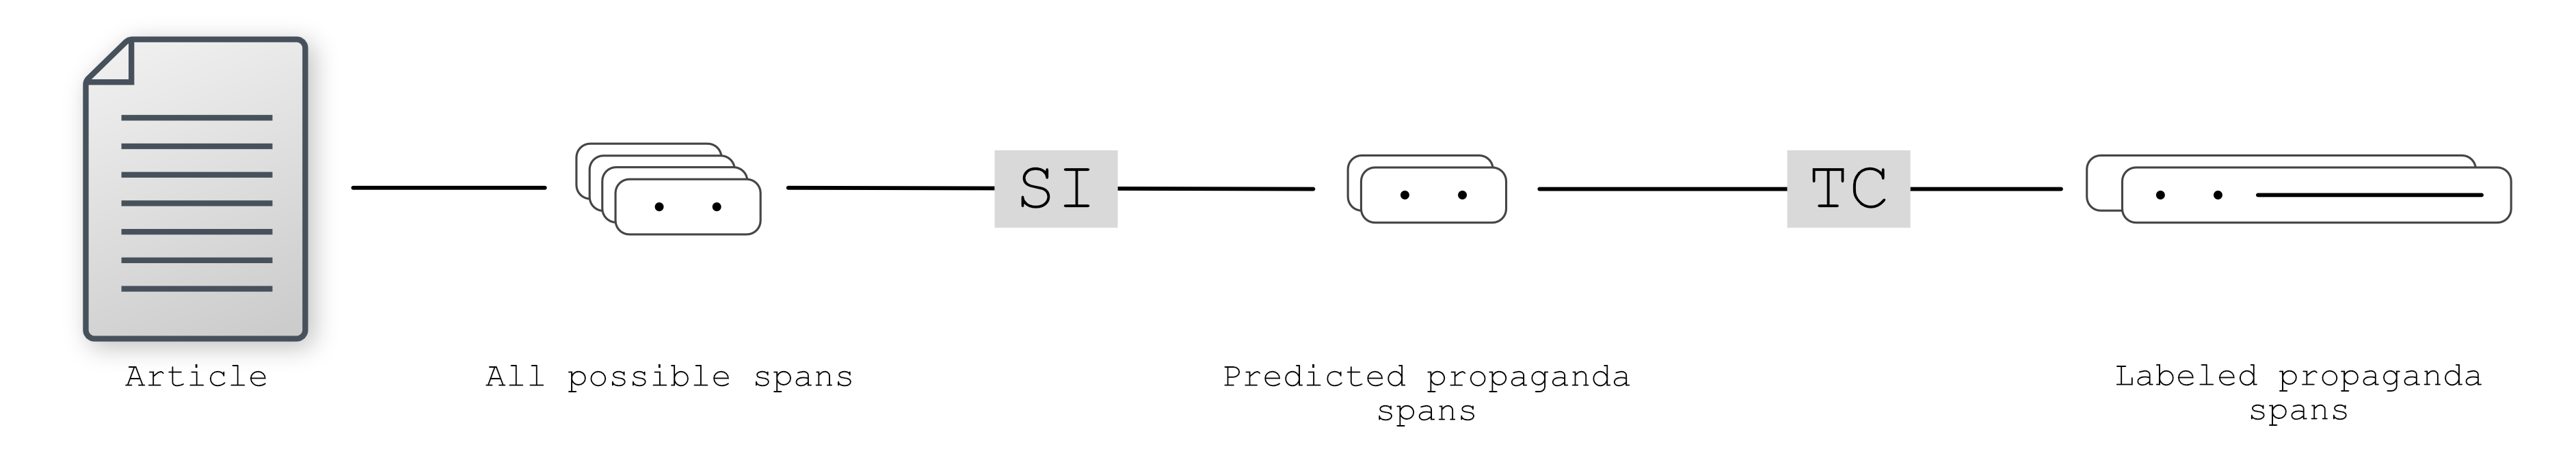
\includegraphics[width=\textwidth]{images/general.png}
    \caption{Overview of the architecture.}
    \label{fig:general}
\end{figure*}

To provide additional means of fine-tuning the final architecture, we also decided to consider the \pol{SI} model as a span classification task rather than a sequence labeling task (see Section \ref{sec:si}). This meant that for each possible span, the \pol{SI} model assigns a probability of being a propagandist argument, and therefore lets the \pol{TC} model only classify spans that have this propaganda likelihood exceeding a well-chosen threshold. 
Intuition was that this would let us regulate the number of false positives we forward onto \pol{TC} and make full use of the slackness offered by the added "\textit{Not Propaganda}" class. 

In this architecture, it could be argued that the addition of this new 15th label renders the \pol{SI} model unnecessary, but its use has strong computational advantages in allowing us to extensively prune the set of considered spans, and to counteract the very heavy class imbalance we would have if we were considering every possible spans in the \pol{TC} task.

\subsection{Span Identification (\pol{SI})} \label{sec:si}
Span identification is often seen as a sequence labeling task, using Begin (\pol{B}), In (\pol{I}) and Out (\pol{O}) labels to classify each token as being in, out, or the beginning of a span. Despite the fact that many teams have used this common technique to model the problem, we decided to go another route and see it as a \textit{span classification} task. This means that we enumerate all possible spans in the article, filtering them with heuristics (see Section \ref{sec:si:preprocesing}), and we classify each of those as being a propaganda span or not. Our reasons for approaching this problem that way are the following:
\begin{itemize}
    \item To be able to use our \pol{SI} model as intended in our general pipeline (see Section \ref{sec:sys-desc}), we need a model that takes a span as input and classifies it as being propaganda or not, whereas a \pol{BIO}-tagging scheme would take a text as input and output the predicted propaganda spans.
    \item Furthermore, as seen in Figure \ref{fig:nb-sentences}, a non-negligible number of gold spans span multiple sentences. In some implementations from other teams, such as \cite{dimov2020nopropaganda}, using the \pol{BIO}-tagging scheme meant they were training a model that worked on each sentence individually, and they had to split gold spans spanning multiple sentences, negatively impacting their model's performance.
\end{itemize}

A detailed overview of the \pol{SI} model can be seen in Appendix \ref{app:si}.


\subsubsection{\pol{SI} Preprocessing}  \label{sec:si:preprocesing}
To deal with the exponential number of spans in an article, we used heuristics to filter-out as many of them as possible. First of all, we only consider spans of 10 tokens or less. According to Figure \ref{fig:nb-tokens}, we can still cover 75\% of the gold spans in our training dataset, while only dealing with a computationally manageable amount of spans when enumerating all possibilities (see discussion Section \ref{sec:discussion} for more information). Second of all, we discard spans that consist exclusively of a combination of determinants, punctuation, space or \pol{EOL} tokens, as we can safely assume those will not be propaganda.

\subsubsection{\pol{SI} Embeddings} \label{sec:si:embedding}
After being extracted, spans are embedded before being fed to the classifier. This embedding, also illustrated in Appendix \ref{app:si}, has three components:
\begin{enumerate}
    \item A weighted average of the word embeddings in the span. The weights used are from a general self-attention vector, masked and re-normalized to only contain the span's words. Expectations were that this would encode a general representation of our span.
    \item The contextualised representation of both of the span's endpoints, concatenated. These vectors are obtained by using a \pol{PLM} to embed the text, and then using a Seq2Seq encoder to contextualise those embeddings, in our implementation a \pol{LSTM}. Our intuition was that the first and last tokens in a span would be particularly important to detect propaganda, e.g. if the span begins and ends with a quotation mark, especially if those are contextualised in respect to the entire text.
    \item Finally, the span width is also encoded.
\end{enumerate}

Our results using different \pol{PLMs} to embed words in our text can be seen in Section \ref{sec:si-results}.

\subsubsection{\pol{SI} Loss function}
We are using the binary cross-entropy (BCE) loss to train our model. The use of the BCE loss is standard in binary classification tasks, but especially relevant in our case. Indeed, since the outputs of the \pol{SI} model will be used to prune spans given to the \pol{TC} model, we are not only interested in the classification but in the actual confidence our model has in it, because we can change the confidence threshold for which we discard spans or not in \pol{TC}. 

A specificity of our approach is also that it is affected by an important imbalance between the two classes. Only a small fraction of the spans that are retrieved by the preprocessing stage effectively contain a propagandist argument. To deal with this problem and prevent the model from classifying every span as not propaganda, we introduce a weight for the positive class in the loss function, defined as follows:
\begin{align*}
    weight_{+} = \frac{\#\ spans\ to\ classify}{\#\ propaganda\ spans}
\end{align*}
% where $s$ is to the number of spans that has to be classified and $g$ is the number of gold spans classified as propaganda.

\subsection{Technique Classification (\pol{TC})} \label{sec:tc}
The \pol{TC} model has to label each element of a set $S$ of spans with one of the 14 existing propaganda techniques. Note that this relies on the important assumption that the model is only provided with a set $S$ of spans which contain a propagandist argument. Recall also that our overall architecture is designed to consider the real-world scenario where this assumption cannot be made (see Section \ref{sec:sys-desc}). Our \pol{TC} model was intended to be built on top of the results of the \pol{SI} model. Consequently, we never have access to the ideal set $S$ but rather a relaxed set $S'$ of spans with the easier-to-satisfy assumption that $S \subset S'$. In order to correctly classify spans, we therefore had to add an extra label "\textit{Not Propaganda}" for spans containing no propagandist argument (i.e. belonging to $S'\backslash S$). An overview of our \pol{TC} implementation can be seen at Appendix \ref{app:tc}.

\subsubsection{\pol{TC} Preprocessing}
The key insight is that we can now think of the \pol{SI} model as applying \textit{an additional pruning} procedure on the set of possible spans.

For each article, we first apply the same preprocessing as we did for the \pol{SI} model. Namely, we enumerate all spans following the same heuristics described in Section \ref{sec:si:preprocesing}. We then use a pre-trained \pol{SI} model to get for each of those spans the probability of it containing a propagandist argument, and prune again according to those and a chosen threshold.

Finally, before training the model, we also had to label the set of span $S$ provided by our \pol{SI} model. For each of the spans $s \in S$ we assigned its original label if the span $s$ had a perfect match with a span in the original \pol{TC} training dataset, or our new \textit{"Not Propaganda"} label otherwise.

\subsubsection{\pol{TC} Embedddings}
After being extracted and pruned according to the results provided by the pre-trained \pol{SI} model, spans are embedded using the same techniques we employed for the \pol{SI} span embedding stage (see Section \ref{sec:si:embedding}).

\subsubsection{\pol{TC} Loss function and metric}
We are using the standard cross-entropy (CE) loss to train our model. As in the \pol{SI} analog, this loss may suffer because of the design of our overall architecture. Indeed, depending on the threshold we set as a hyperparameter to filter the spans according to the results of the \pol{SI} model in the \pol{TC} preprocessing, we still could have much more false positives than real propaganda spans. This could lead to an important class imbalance and skew our model's predictions.

To deal with this problem and prevent the model from classifying each of the new spans with the 15th label "\textit{Not Propaganda}", we introduced weights in the loss function. Those weights were assigned in inverse proportion to the distribution of original classes in the dataset (shown in Figure \ref{fig:tech_distr}) and the ratio $r = 0.05$ of spans provided by \pol{SI} model that exactly match a propaganda argument (pointed out in Table \ref{table:iou}). The 15th class proportion is $1-r = 0.95$ and the 14 original classes proportions are $\frac{w_c}{s}$ where $s = \frac{1}{r} \sum_c w_c$ and $w_c$ is their original distribution. We finally reversed the proportions $p_i$ by assigning to each of the classes $1-p_i$ in order to have the final weights.

% We set a weight $w_c$ for each original class, according to the distribution observed in the dataset, shown in Figure \ref{fig:tech_distr}. We then computed the weight of the 15th additional class as $s(1-r)$ where $r$ is the ratio of spans provided by \pol{SI} model that contains a propaganda argument, namely $0.05$, as pointed out in table \ref{table:iou} and $s = \frac{1}{r} \sum_c w_c$ is a normalization constant ensuring our weights form a valid distribution over our classes. Finally every weight was divided by the normalization factor $s$ to ensure the distribution sums up to $1$.

\section{Experiments}

\subsection{\pol{SI} results} \label{sec:si-results}
The metric used to evaluate our \pol{SI} model is a custom F$_1$-measure that allows non-zero scores for partial matches between predicted and gold spans, as proposed in \cite{semeval}. The rest of the experimental setup can be seen in Table \ref{table:si-params}.

\begin{table}[h]
\centering
  \begin{tabular}{c c}
    \hline
    \textbf{Hyperparameter} & \textbf{Value} \\
    \hline
    Epochs & 10 \\
    Batch size & 1 \\
    Max span width & 10 \\
    Max sequence length & 128 \\
    \pol{LSTM} dimension & 200 \\
    Learning rate (LR) & 1e-3 \\
    Transformer LR & 1e-5 \\
    \hline
  \end{tabular}
  \caption{Experimental setup for \pol{SI}.}
  \label{table:si-params}
\end{table}

As discussed in Section \ref{sec:discussion}, our setup, and therefore our results, were heavily influenced by various limitations. Even though, \pol{SI} achieved good results. \pol{RoBERTa} obtains the highest F$_1$ score on the test set, as reported in Table \ref{table:si-test-results}, letting us rank 8th out of 45 teams. 

\begin{table}[h]
\centering
  \begin{tabular}{|c|c c c|}
    \hline
    \textbf{Model} & \textbf{Custom F\textsubscript{1}} & \textbf{Precision} & \textbf{Recall} \\
    \hline
    \pol{\textbf{BERT}} & 0.40008 & 0.29371 & 0.62722 \\
    \pol{\textbf{RoBERTa}} & 0.42649 & 0.32754 & 0.61107 \\ 
    \pol{\textbf{XLNet}} & 0.37930 & 0.26213 & 0.68590 \\
    \hline
  \end{tabular}
  \caption{Model results on \pol{SI} task on validation data.}
    \label{table:si-val-results}
\end{table}

\begin{table}[h]
\centering
  \begin{tabular}{|c|c c c|}
    \hline
    \textbf{Model} & \textbf{Custom F\textsubscript{1}} & \textbf{Precision} & \textbf{Recall} \\
    \hline
     \textbf{\pol{BERT}}  & 0.29651 & 0.17528 & 0.96147\\ 
    \textbf{\pol{RoBERTa}}  & 0.46072 & 0.40635 & 0.53189 \\
    \textbf{\pol{XLNet}}  & 0.43133 & 0.50394 & 0.37701\\
    \hline
  \end{tabular}
  \caption{Model results on \pol{SI} task on test data.}
    \label{table:si-test-results}
\end{table}

\subsection{\pol{TC} results} \label{sec:tc-results}
Even if our novel approached seemed reasonable on paper, the results of the experiments conducted with it clearly pointed to the opposite direction. The assumption that \pol{SI} returns a set of spans containing all the gold spans was not respected, as discussed in Section \ref{sec:si-error-analysis}. The problem being that a \textit{perfect match} with a gold span is rarer than expected (see Table \ref{table:iou}). Therefore, during training, when generating the labels for the spans provided by the \pol{SI} model, we didn't often have a perfect match and thus all our training samples were labelled as \textit{"Not propaganda"} (because of our strategy to generate gold labels, as discussed in Section \ref{sec:tc}). This was preventing our algorithm from learning to distinguish between our classes. Indeed, the model output the "\textit{Not Propaganda}" class for every span.

\subsubsection*{Partially overlapping \pol{TC}}
In order to counteract this limitation, we tried to further relax our model and enrich our gold labels set with \textit{partially overlapping} spans (as described in Table \ref{table:error-si-tech}). For instance, if \pol{SI} predicts a span $s$ spanning from token $12$ to token $26$ and there is a gold span going from token $13$ to token $27$ with label $l$, we assigned this propaganda label $l$ to the span $s$ provided by \pol{SI}. We thus enriched our dataset with partially overlapping spans according to some threshold. However, this method was not successful either in practice, still leading to a model that predicted "\textit{Not Propaganda}" for every span. Indeed, as shown in Table \ref{table:iou}, even going as far as allowing for 50\% of the span to be a false positive, we would only get 20\% of labels being something other than "\textit{Not Propaganda}" in our training set, which was not enough to overcome the issue.

\subsubsection{Alternative \pol{TC} results}
To demonstrate the individual abilities of our \pol{TC} model, we finally decided to implement an alternative version of \pol{TC}, not taking as input the set of spans provided by our \pol{SI} model, but taking the spans directly from the dataset as initially proposed by the organizers i.e. a perfectly pruned set of spans. We also removed our 15th class "\textit{Not Propaganda}". This alternative \pol{TC} demonstrated that our two modules can nevertheless work independently and are capable of providing decent results on both sub-tasks.


\begin{table}[h]
\centering
  \begin{tabular}{c c}
    \hline
    \textbf{Hyperparameter} & \textbf{Value} \\
    \hline
    Epochs & 1 \\
    Batch size & 1 \\
    Max span width & 10 \\
    Max sequence length & 128 \\
    \pol{LSTM} dimension & 200 \\
    Learning rate (LR) & 1e-3 \\
    Transformer LR & 1e-5 \\
    \hline
  \end{tabular}
  \caption{Experimental setup for \pol{TC}.}
  \label{table:tc-params}
\end{table}

The metric used to evaluate the TC model is a standard micro-averaged F$_1$-measure, and the exact experimental setup is the same as for our other \pol{TC} model, and can be seen in Table \ref{table:tc-params}. 

Training with \pol{RoBERTa}, we achieved a validation F$_1$ metric of $0.57572$. Notice that we were not able to generate results for the test data. Because the model took as input the gold spans to be predicted by the \pol{SI} model, the organizers of the task decided to not share them publicly. After contacting them, we were not able to get access to the correct file in time. Although this is the case, because no hyperparameters were tuned, our validation data serves the same purpose as a test dataset, and should be representative of our model's performance on inputs not seen during training.


\begin{table*}[t]
\centering
  \begin{tabular}{c r c c c c c c c c c c c c c c c c c c c }
  
    & \rotatebox{90}{  Loaded Language}
    & \rotatebox{90}{  Name Calling }
    & \rotatebox{90}{  Repetition }
    & \rotatebox{90}{  Flag Waving }
    & \rotatebox{90}{  Exaggeration }
    & \rotatebox{90}{  Doubt }
    & \rotatebox{90}{  Prejudice }
    & \rotatebox{90}{  Slogans }
    & \rotatebox{90}{  Red Herring }
    & \rotatebox{90}{  Appeal to Authority }
    & \rotatebox{90}{  Reductio ad hitlerum }
    & \rotatebox{90}{  Oversimplification	}
    & \rotatebox{90}{   Cliches	}
    & \rotatebox{90}{  Authority}
    & Total \\
    \hline
    Not identified & 51& 35&  56& 18& 28&  42& 9& 10&  17&  7& 4 & 13& 9& 7& 306\\
    Partially identified & 23&  18& 3& 19&  12& 18& 17& 4&  8&  1& 1 & 4& 3& 1& 132 \\
    Totally identified & 251&  130& 86& 50& 28& 6& 18& 26&  4& 6& 0 & 1 & 5& 6& 617 \\
    \hline
    Total & 325& 183& 145& 87& 68& 66& 44& 40& 29&  14& 5 & 18 & 17 & 14 & 1055\\
    \hline

  \end{tabular}
  \caption{\centering \pol{SI} results broken down by propaganda technique. In this setting, a gold span was considered \textit{totally identified} if at least 75\% of its characters were labeled as propaganda, \textit{partially identified} if a percentage between 15\% and 75\% of its characters were labeled as propaganda, \textit{not identified} if less than 15\% of its characters were labeled as propaganda.} 
    \label{table:error-si-tech}
\end{table*}

\section{Error analysis}
In order to draw meaningful conclusions about proposed architectures and their performances on both sub-tasks, a specific in-depth error analysis was conducted. 

This analysis was performed on classification results of the top performing model for each task, namely \pol{RoBERTa-si} and \pol{RoBERTa-tc}. The data used as benchmark was validation data — since no hyperparameter tuning was performed on them (except for the choice of \pol{PLM}) and therefore they could be used to obtain unbiased information.

\subsection{Span Identification Task} \label{sec:si-error-analysis}
As a first approach to the error analysis for \pol{SI} task, we decided to further investigate the results by breaking them down by propaganda technique. Although, in this task, the model does not explicitly deal with technique classification, all propaganda spans still belong to a specific category, and analysis of how it influenced the prediction results was considered potentially insightful.

Moreover, since the custom F$_1$ metric used in \pol{SI} allows non-zero scores for partial matches, the proportion between partially classified, totally identified and entirely missed propaganda spans in the validation articles were included in the analysis. The results of this investigation are reported in Table \ref{table:error-si-tech}. 

As the data highlights, our system was unable to identify almost one third of propaganda spans in the given articles. On the other hand, roughly $60\%$ of the spans were \textit{totally identified} (i.e. with more than 75\% of the characters being correctly classified by \pol{SI} as propaganda). However, the high disproportion between partial matches and complete matches, together with the higher \textit{recall} value than \textit{precision} registered in both validation and test results, might suggest that our system tends to predict larger spans than necessary.

An important remark that has to be made is about the changes between the proportion of identified and not identified spans in more (e.g. \textit{Loaded Language} and \textit{Name Calling}) and less (e.g. \textit{Red Herring} and \textit{Reductio ad hitlerium}) frequent techniques. This trend could suggest a direct relation between the number of instances for each propaganda technique and the accuracy achieved by the system in correctly classifying a span that belongs to that technique. This relation can be observed in Figure \ref{fig:tech-dist-si}, which reports the distribution of identification proportion for different propaganda techniques.\\

\begin{figure}[h]
    \centering
    \begin{subfigure}{0.23\textwidth}
        \centering
        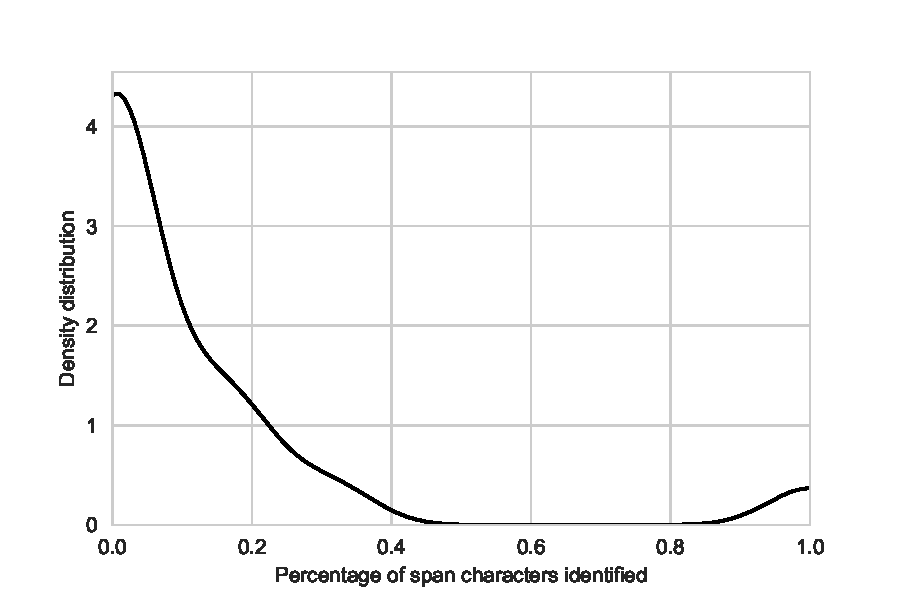
\includegraphics[width=\linewidth]{images/Causal_Oversimplification.pdf}
        \caption{Causal Oversimplification}
        \label{subfigure:oversim}
    \end{subfigure}
    \begin{subfigure}{0.23\textwidth}
        \centering
        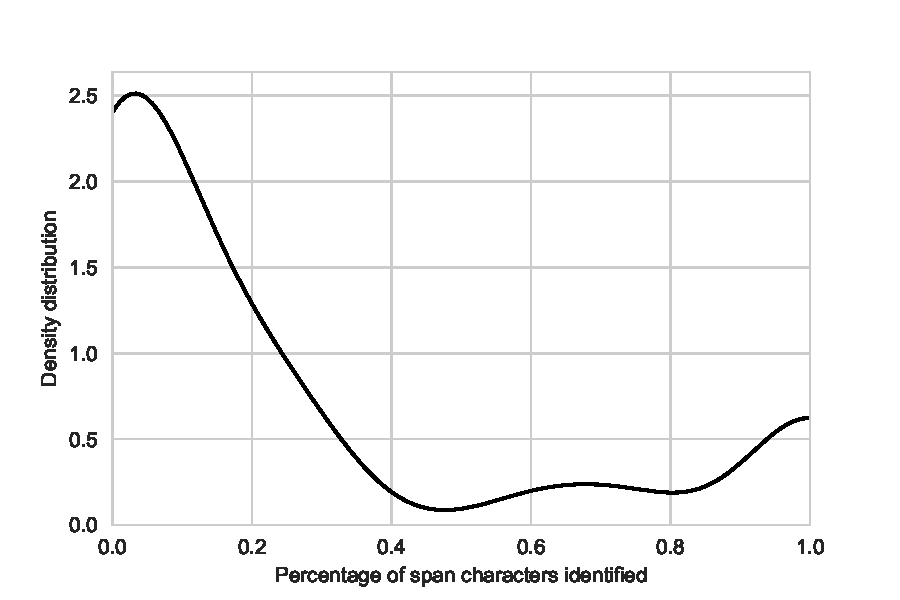
\includegraphics[width=\linewidth]{images/Red_Herring.pdf}
        \caption{Red Herring}
        \label{subfigure:red}
    \end{subfigure}
    \begin{subfigure}{0.23\textwidth}
        \centering
        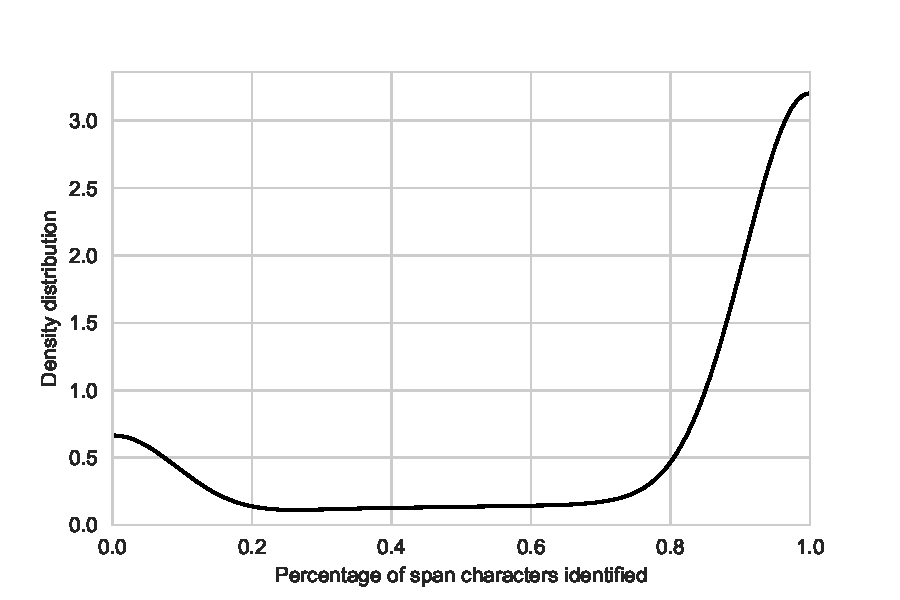
\includegraphics[width=\linewidth]{images/Loaded_Language.pdf}
        \caption{Loaded Language}
        \label{subfigure:loaded}
    \end{subfigure}
    \begin{subfigure}{0.23\textwidth}
        \centering
        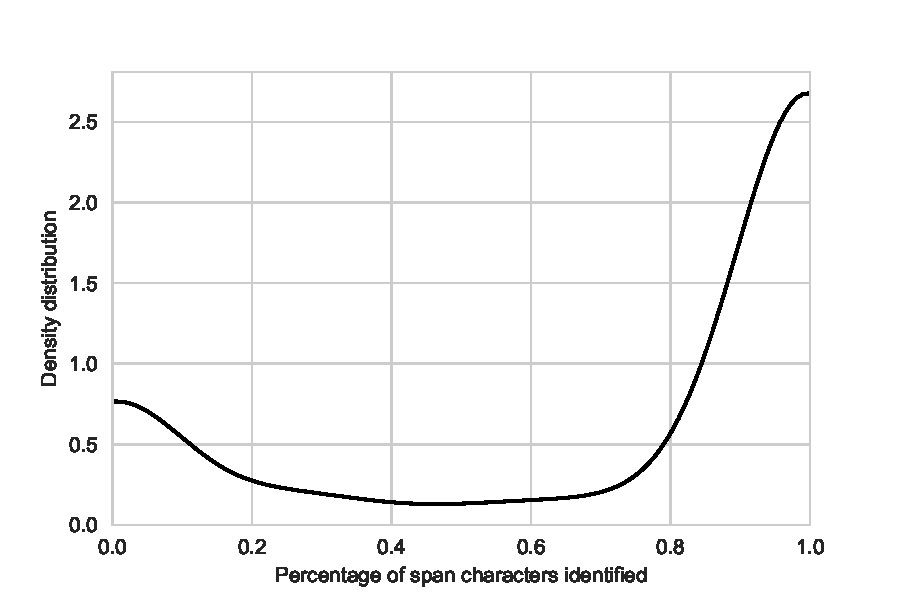
\includegraphics[width=\linewidth]{images/Name_Calling.pdf}
        \caption{Name Calling}
         \label{subfigure:calling}
    \end{subfigure}
    \caption{Distribution of identification percentage of gold spans which belong to four different propaganda technique. It can be observed how less frequent techniques in the training set (Figures \ref{subfigure:oversim} and \ref{subfigure:red}) are much harder to label compared to more frequent techniques (Figures \ref{subfigure:loaded} and \ref{subfigure:calling}).}
    \label{fig:tech-dist-si}
\end{figure}

However, data in Table \ref{table:error-si-tech} is not enough to completely characterize the quality of the predictions of the proposed \pol{SI} model. Because of this, a more in-depth analysis on the similarity between predicted propaganda spans and gold spans was conducted. To evaluate the similarity between predicted spans and gold spans the metric Intersection over Union (\pol{IoU}) was used. \pol{IoU}, also known as \textit{Jaccard index} or \textit{Jaccard similarity coefficient}, is a statistic used for gauging the similarity and diversity of sample sets. It is defined as the size of the intersection divided by the size of the union of the sample sets (i.e. text spans in our setting):

\begin{align*}
    IoU(S_1,S_2) = \frac{|S_1 \cap S_2|}{|S_1 \cup S_2|} 
\end{align*}

The analysis was performed by aggregating all predicted spans which matched different thresholds of score, to gain better insights on the distribution of likelihood of our predictions with respect to gold labels. The results of this study are reported in Table \ref{table:iou}. As we can see from the data, just a very small percentage of the predicted labels \textit{perfectly} match a gold label, and in this behaviour lies one of the biggest weakness of our proposed architecture. Here we see that one of the fundamental assumption of the proposed approach, that the gold spans are a subset of the predicted spans from \pol{SI}, does not hold in practice.

\begin{table}[h]
\begin{tabular}{ |c | c| c| c| c| } 
\hline
 \textbf{Threshold} & 1 & $\geq 0.5$ & $\geq 0.25$ & $ > 0$ \\ 
\hline
\textbf{Percentage} & 0.041 & 0.205 & 0.301 & 0.397 \\
 \hline
\end{tabular}
\caption{Percentages of predicted spans which match different values of \pol{IoU} score.}
 \label{table:iou}
\end{table}

\subsection{Technique Classification Task}
As already mentioned in Section \ref{sec:tc-results}, the \pol{TC} model implemented following the novel approach proposed in this project was not able to produce meaningful results for the Technique Classification sub-task. Indeed, performing an error analysis on the results produced by this model would not be interesting.

However, it was still possible to investigate the results obtained with the alternative \pol{TC} classifier. Figure \ref{fig:confusion-mat} reports the normalized confusion matrix obtained from the analysis of the model prediction on validation data. Interestingly, the most confused classes are \textit{Exaggeration} (primarily with \textit{Loaded Language}), \textit{Doubt} (in this case, mainly with \textit{Repetition}) and \textit{Prejudice} (primarily with \textit{Loaded Language} and \textit{Authority}).

It is also worth observing that, unfortunately, many less-frequent propaganda techniques does not appear in the validation set, and is therefore impossible to have an unbiased evaluation of the classification performances for those techniques.

\begin{figure}[h]
    \centering
    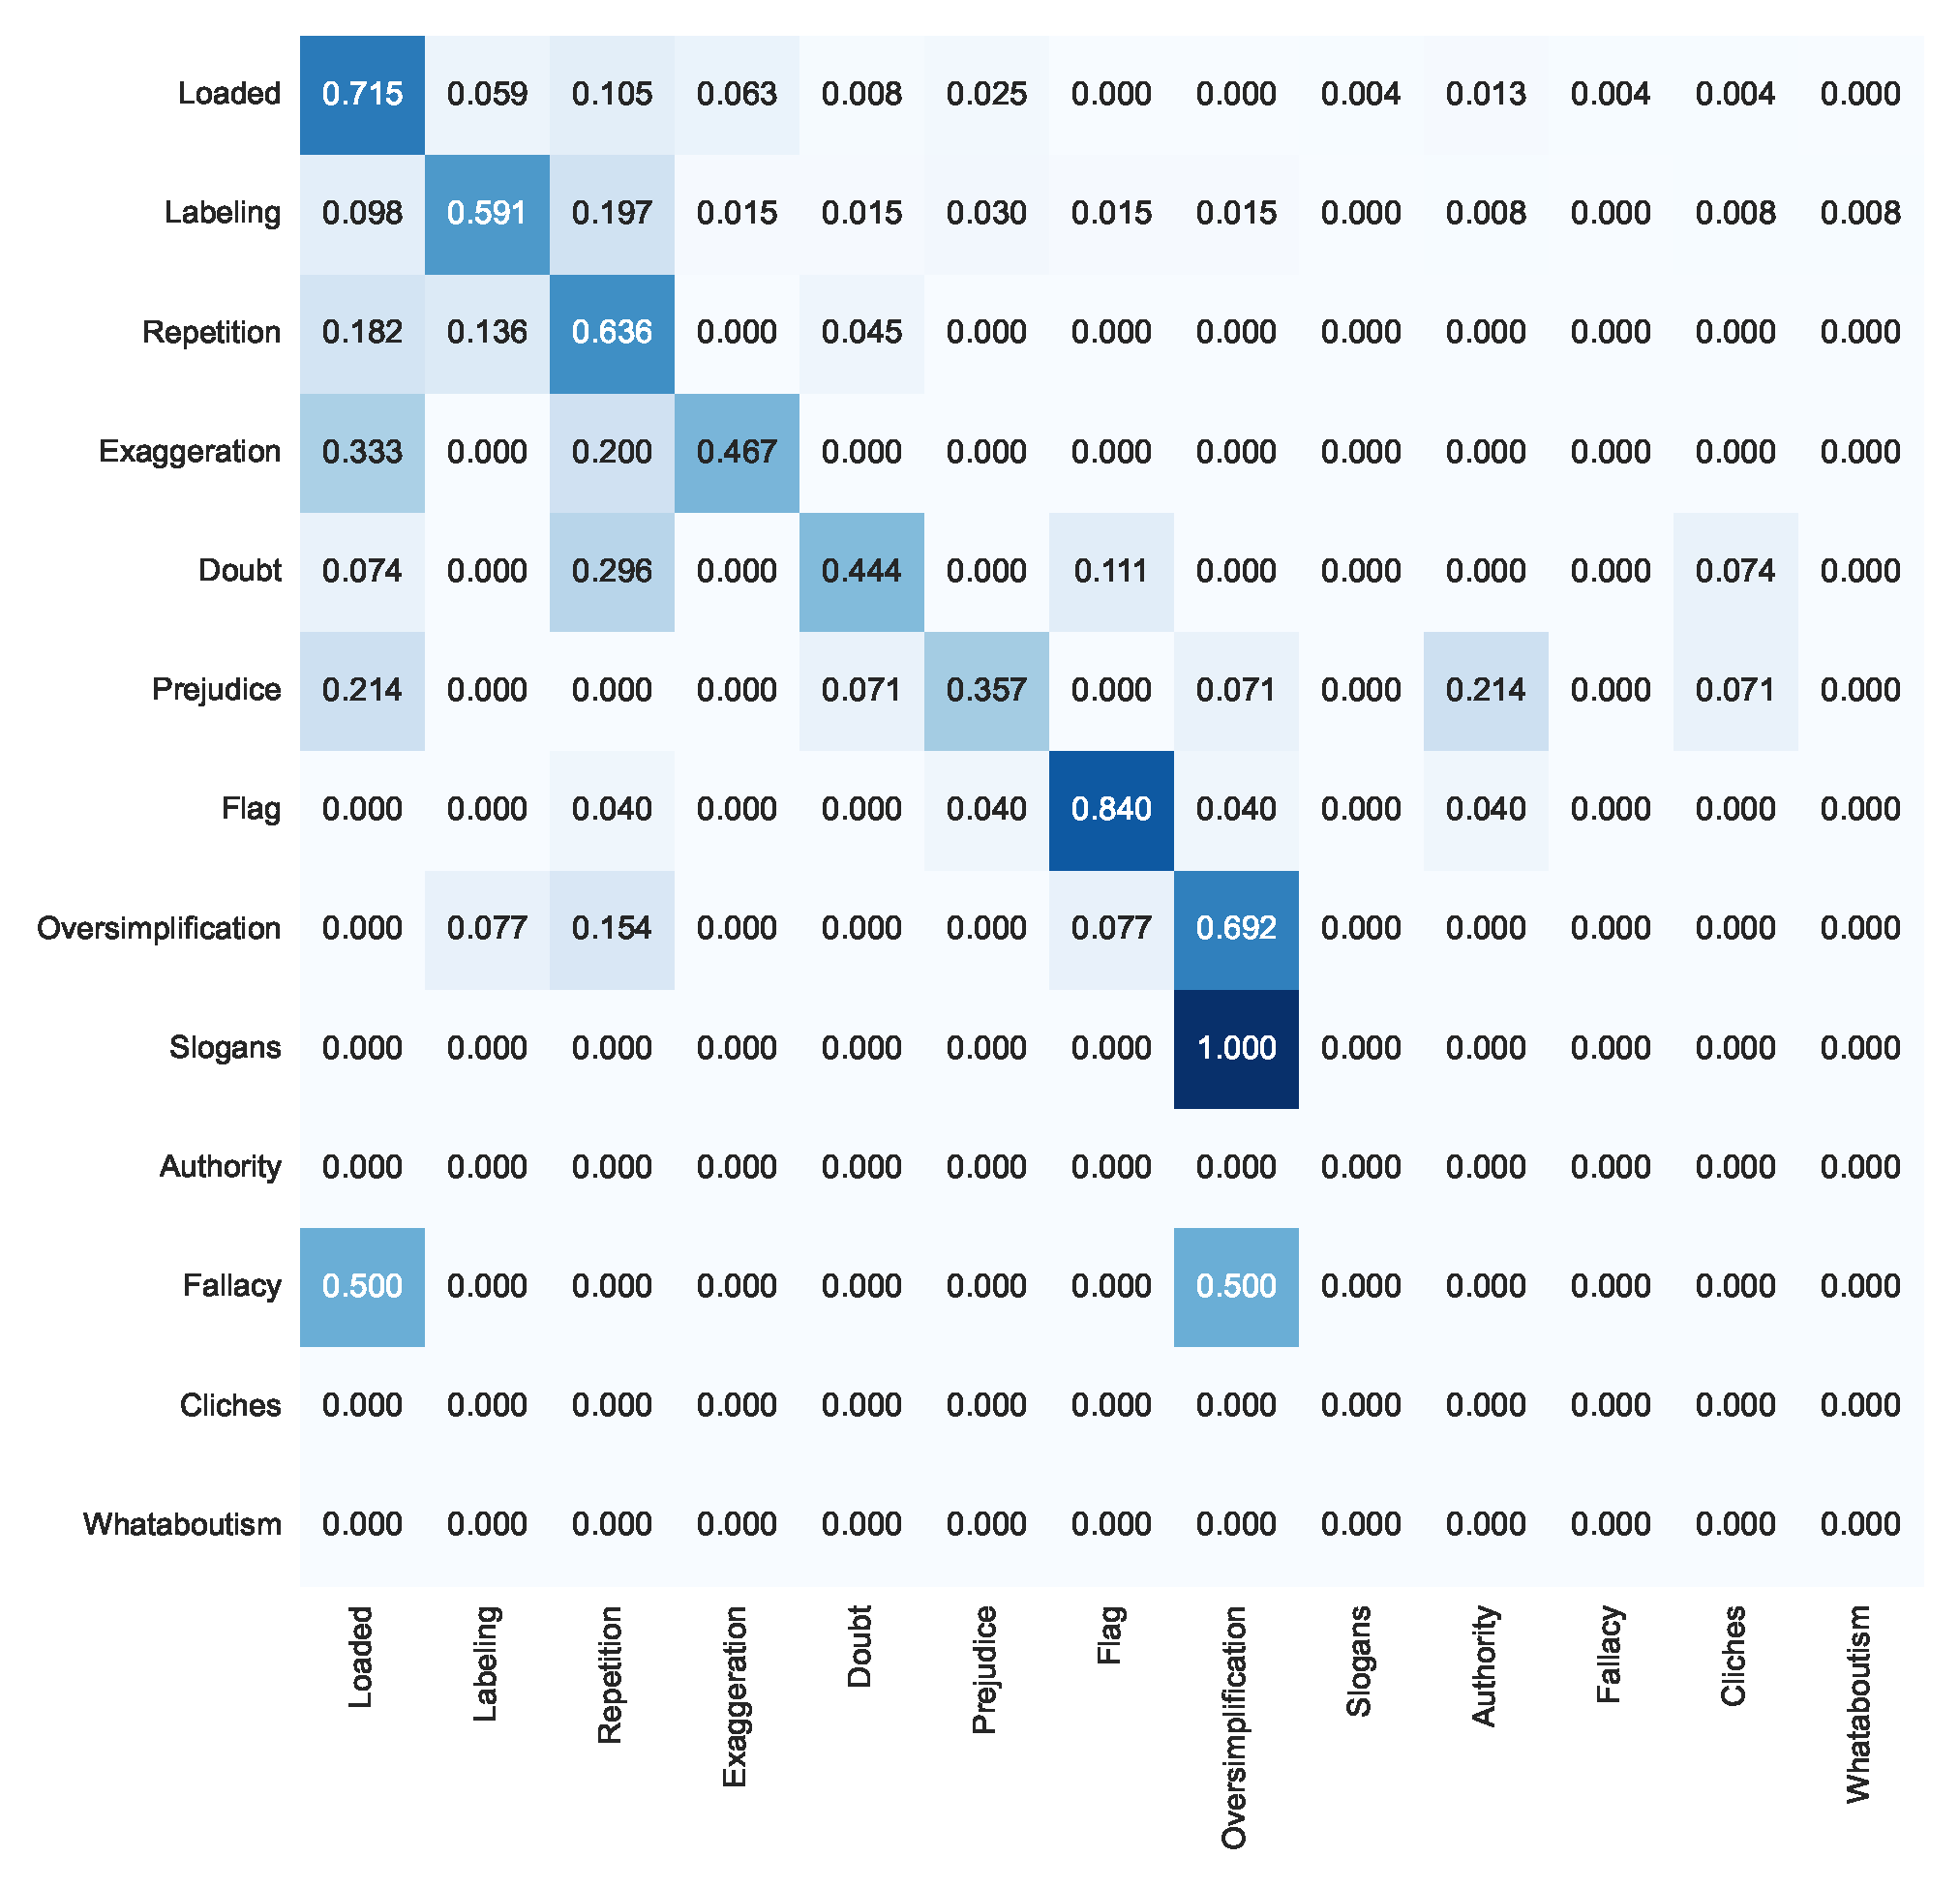
\includegraphics[width=0.45\textwidth]{images/confusion.pdf}
    \caption{Normalized confusion matrix obtained from results of alternative \pol{TC}. Rows represent the correct labels and columns the predicted ones.}
    \label{fig:confusion-mat}
\end{figure}

\section{Discussion and summary}
\subsection{Discussion} \label{sec:discussion}
In this work, a novel approach to tackle the detection and classification of propaganda spans in news article was investigated. The core idea behind it was to develop a tool that would have been able to better adapt to real-world scenarios. 
Nonetheless, during the development of this tool many flaws were found in the initial approach, that proved to not be as effective as initially expected.

The first problem faced during the development of \pol{SI} regarded the memory complexity of the approach. As already mentioned, the decision to approach the task as a span classification problem lead to the evaluation of a potentially exponential number (in the size of the article) of sequences. This, other than the obvious problem with class imbalance between propaganda and non-propaganda spans, also resulted in a major memory issue with batch embedding computation. 
The memory issue prevented us from effectively training our models on GPUs — due to the limited memory available. This forced us to train our models on CPUs, which resulted in slower computations and therefore the impossibility to perform hyperparameter tuning and validation of our models with techniques like cross-validation and statistical significance indices.

The second problem was the predicting efficiency of our \pol{SI} model. In the proposed approach the efficiency of \pol{TC} was relying on a good span extraction from \pol{SI}. Since the experiments proved our necessary assumption to be wrong, as discussed in Section \ref{sec:si-error-analysis}, the \pol{TC} model could not provide satisfactory results.

However our \pol{SI} model still predicts propaganda spans relatively well, even if it does not give exact matches. Proof of this is the test result achieved with \pol{RoBERTa} and our rank in the leaderboard ($8 / 45$). Furthermore, our alternative for the \pol{TC} task achieves an F$_1$ metric of $0.57572$, and supports the idea that our original model for \pol{TC} is inherently flawed and not that its failure is due to some implementation error.

\subsection{Future work}
Because of the context of this project, and the time limit associated with it, we were not able to implement all of the ideas we had to improve our model. To build upon our work, we propose to look into the following:
\begin{itemize}
    \item Fine-tuning our investigated models using different \pol{PLM}s, changing hyper-parameters and adding regularization methods. 
    \item The exploration of add-on features for the architecture such as conditional random field.
    \item The error analysis revealed that the propaganda techniques commonly confused in the \pol{TC} task are the same as the techniques that our model was unable to detect in the \pol{SI} task. A possible route of improvement for the latter might be deploying data augmentation techniques (such as back translation, random replacement and random insertion) to enrich the number of samples that belongs to less frequent techniques, in order to facilitate their identification.
    \item Improving our top layer classification algorithm. For the models studied, we explored only linear classification and it might be possible to achieve better results with deeper networks.
    \item Exploring more \pol{PLMs} and eventually using ensemble techniques to get even more meaningful embeddings.
\end{itemize}

\subsection{Outro}
This very paper, as well as the ETH Zürich Natural Language Processing course's lectures note, were checked using the proposed system, to detect fragments one may suspect to represent one or more propaganda techniques. The results are included in Appendix \ref{app:preds}.

% To add references without citing in text
\nocite{*}

% Entries custom bib
\bibliography{custom}
\bibliographystyle{acl_natbib}

\clearpage
\pagebreak

\onecolumn
\begin{appendices}


\section{\pol{SI} model detailed architecture} \label{app:si}
\begin{figure}[h]
    \centering
    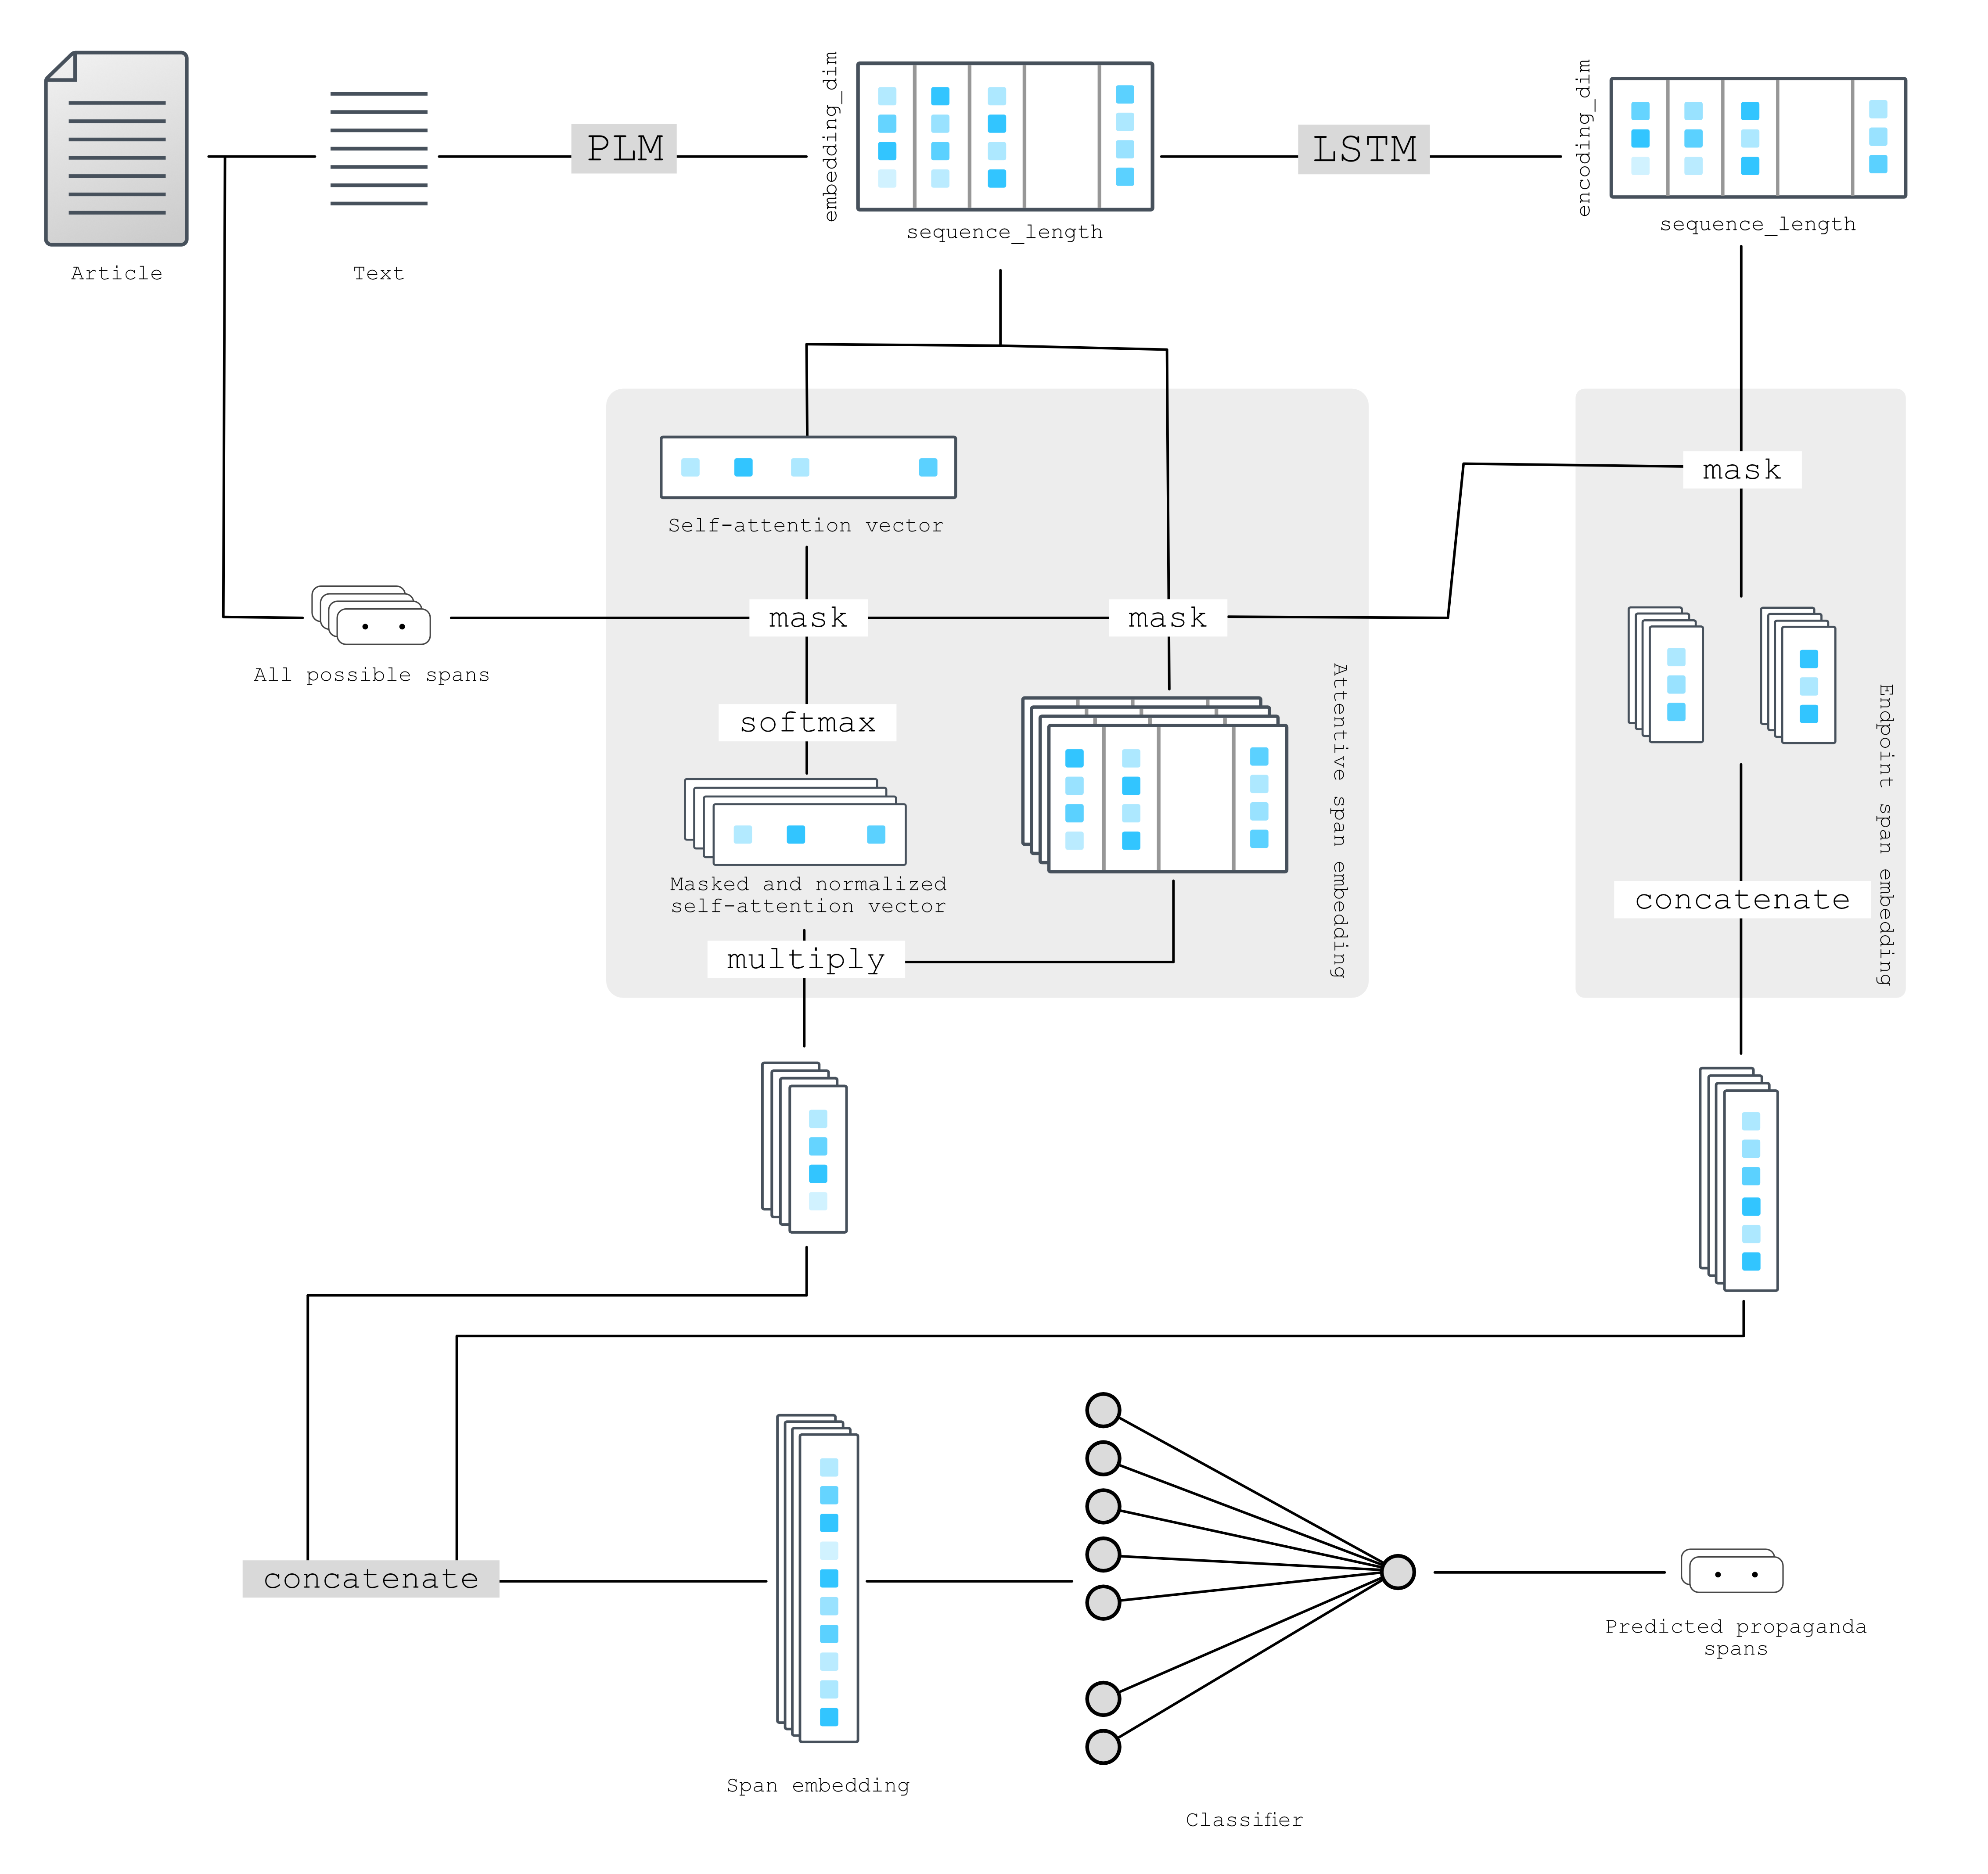
\includegraphics[width=\textwidth]{images/si.png}
    \label{fig:si-architecture}
    \caption{Some illustrations from the \pol{AllenNLP} guide.}
\end{figure}

\clearpage
\pagebreak
\section{\pol{TC} model detailed architecture} \label{app:tc}
\begin{figure}[h]
    \centering
    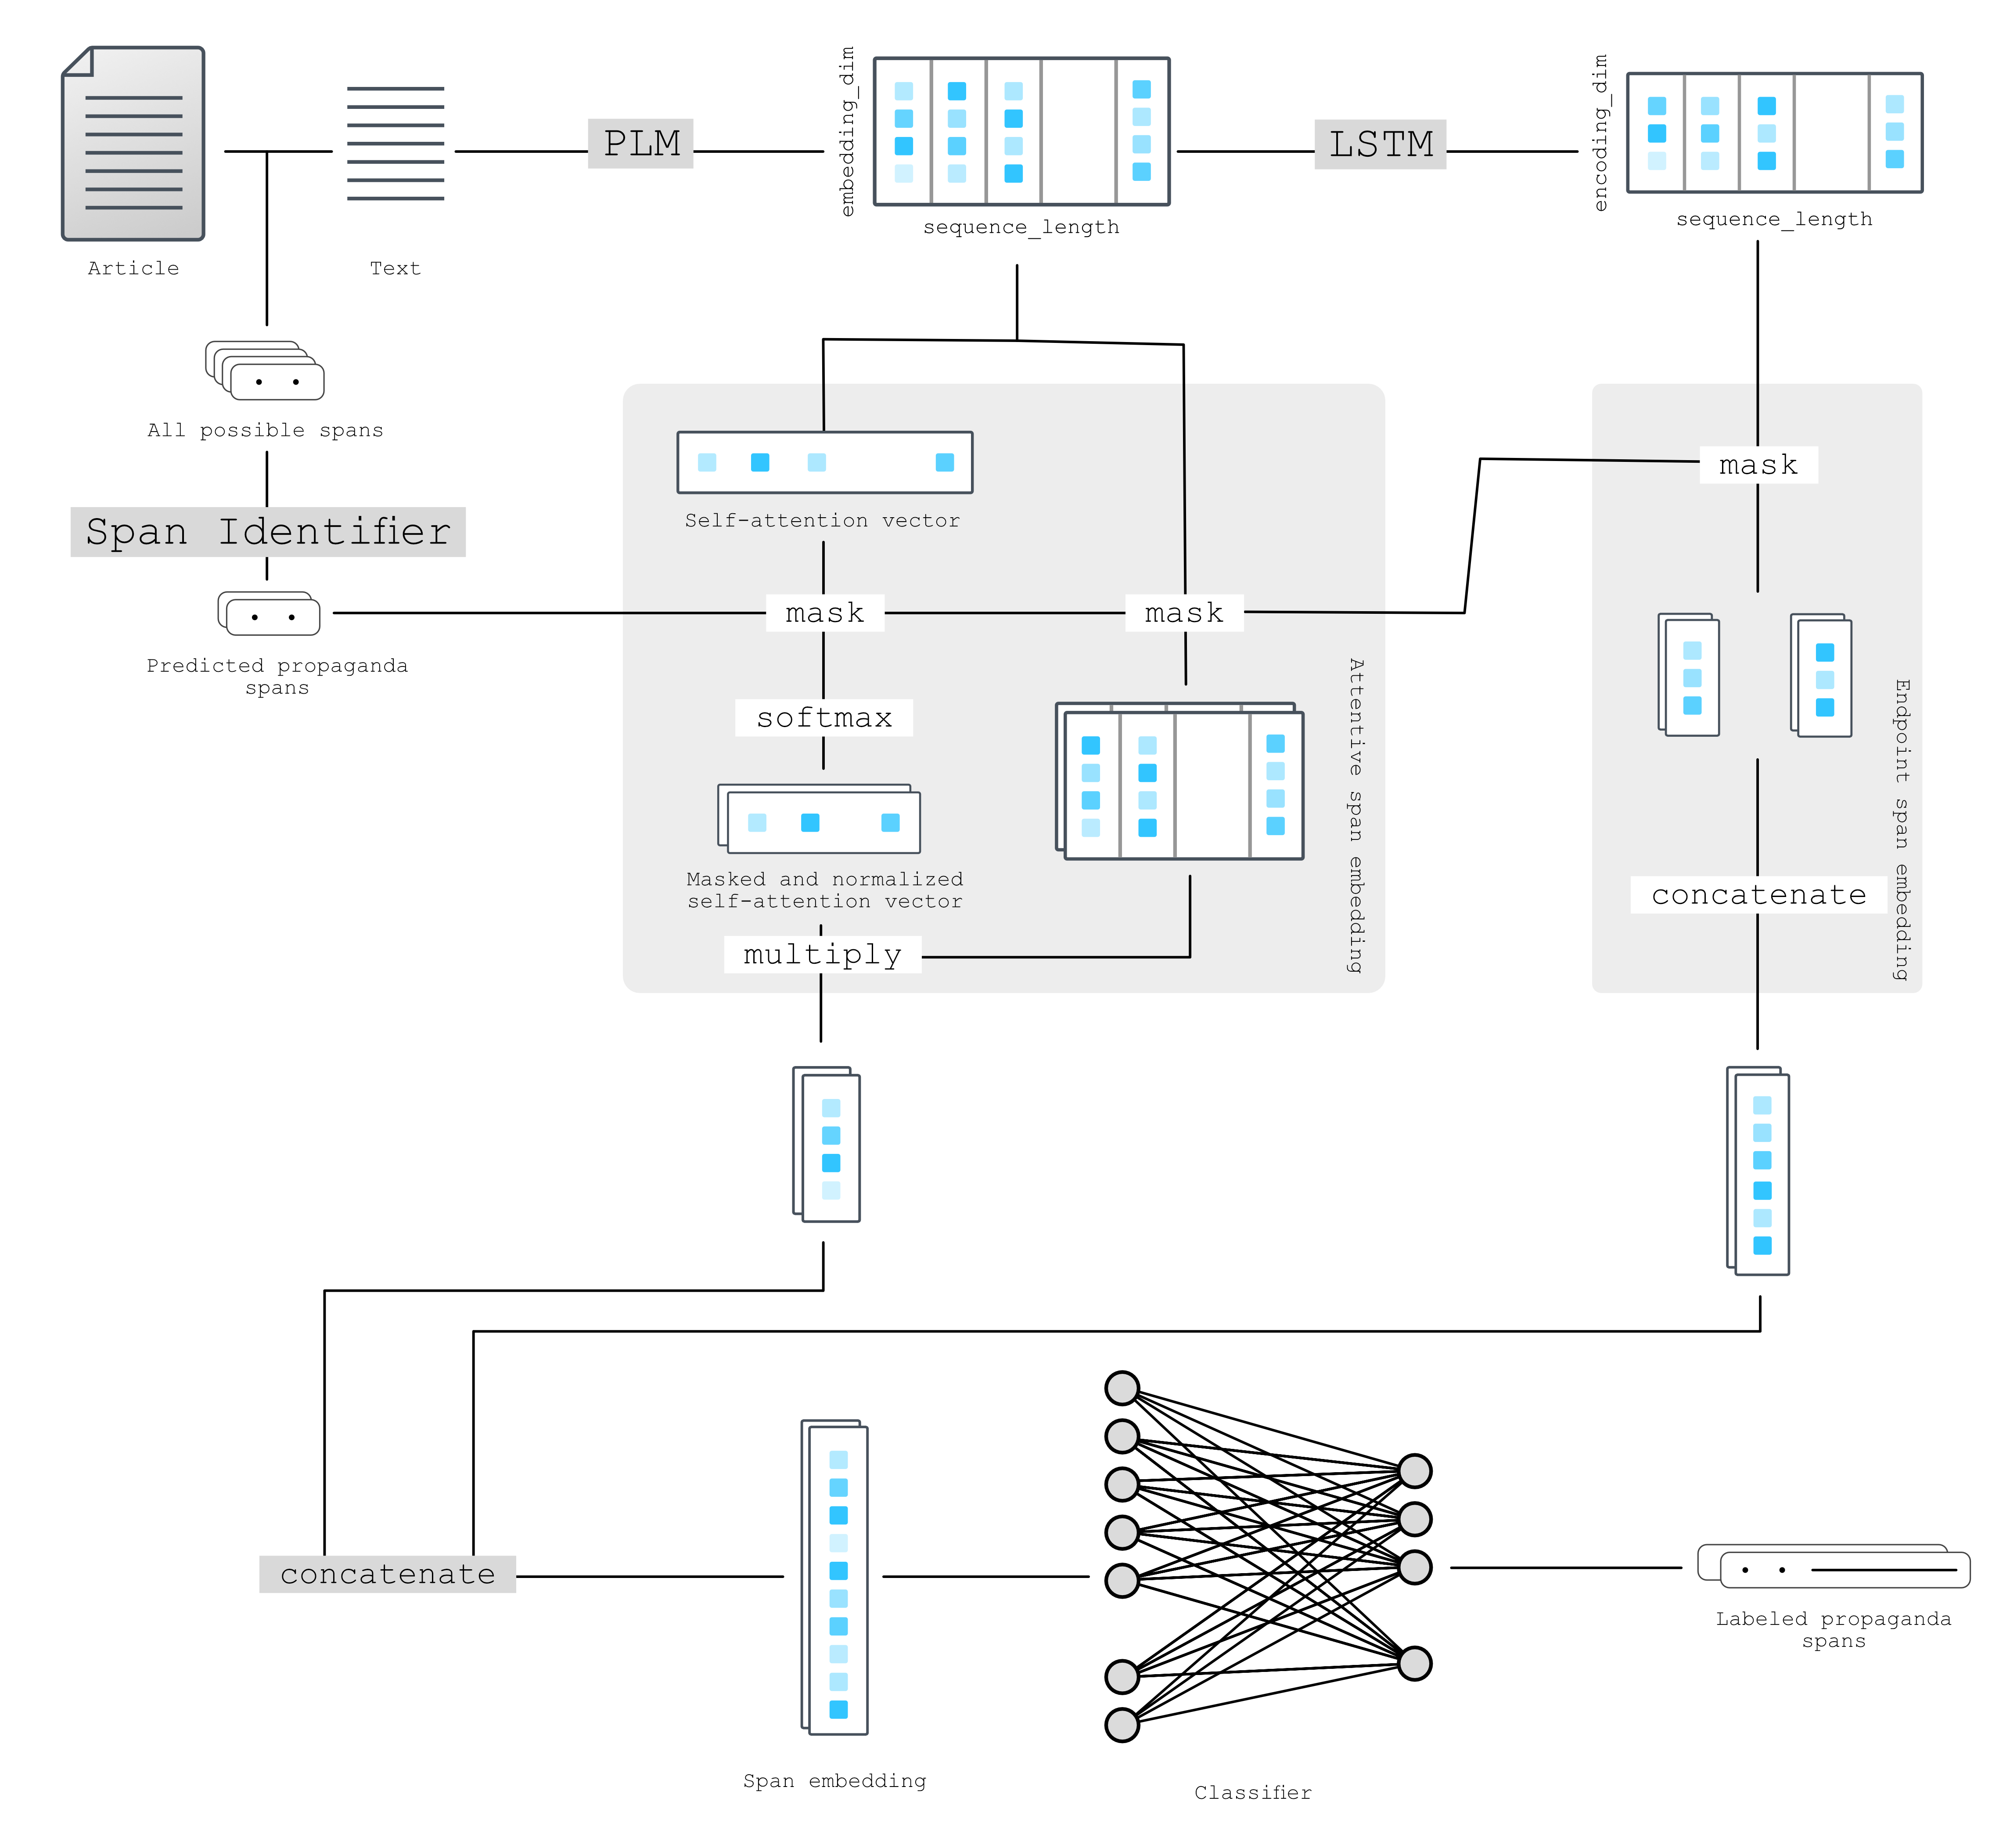
\includegraphics[width=\textwidth]{images/tc.png}
    \label{fig:tc-architecture}
    \caption{Some illustrations from the \pol{AllenNLP} guide.}
\end{figure}

\clearpage
\pagebreak
\section{Predictions on lecture notes and this paper} \label{app:preds}

\subsection{Propaganda detection on the NLP Course notes\footnote{\url{https://drive.google.com/file/d/1esgbEGgF2TYwr0wCE5Sb18YLJ3A9eDgp/view}}}

\footnotesize
\begin{verbatim}
highly inefficient	Loaded_Language
comes in handy .	Loaded_Language
redundancies .	Loaded_Language
cumbersome	Loaded_Language
the sleeker zn .	Name_Calling,Labeling
inductive hypothesis )	Loaded_Language
exponential	Loaded_Language
redundant .	Loaded_Language
the magic of backpropogation .	Loaded_Language
the cheap gradient principle :	Name_Calling,Labeling
cheap	Loaded_Language
log - linear models	Repetition
analytically tractable .	Loaded_Language
log - linear ,	Name_Calling,Labeling
completely BROKEN ! "	Loaded_Language
broken ,	Loaded_Language
spam classification example	Name_Calling,Labeling
gradient descent .	Loaded_Language
log - softmax ,	Name_Calling,Labeling
exponential families .	Repetition
our estimate ,	Loaded_Language
very convenient	Loaded_Language
The crux of the argument	Loaded_Language
non - linear boundary ?	Name_Calling,Labeling
log - linear models	Name_Calling,Labeling
non - linear decision boundaries , by	Repetition
log - linear models :	Name_Calling,Labeling
vanishing gradients .	Loaded_Language
one - hot encoding scheme .	Name_Calling,Labeling
skip - gram model	Repetition
naive computation	Loaded_Language
structured prediction .	Repetition
structured prediction task ,	Repetition
bigram language model	Loaded_Language
bigram assumption	Loaded_Language
smoothing .	Loaded_Language
neural n - gram models	Name_Calling,Labeling
log - linear models	Name_Calling,Labeling
illustrating example	Loaded_Language
inherently limited	Loaded_Language
explode	Loaded_Language
I duck “	Repetition
A duck “ ,	Name_Calling,Labeling
shortest - path - search problem	Loaded_Language
computationally intractable .	Loaded_Language
our problem .	Flag-Waving
additively decomposable	Loaded_Language
additively decomposable ,	Loaded_Language
an annihilator	Name_Calling,Labeling
semirings	Loaded_Language
overwhelming evidence	Loaded_Language
structured hierarchically .	Loaded_Language
hierarchical nature	Loaded_Language
caviar	Loaded_Language
a cleft sentence ,	Loaded_Language
How does papa eat caviar ?	Doubt
With a spoon ]	Loaded_Language
red car ”	Repetition
red car ”	Repetition
red car ”	Name_Calling,Labeling
single - root constraint .	Name_Calling,Labeling
projective and non - projective .	Repetition
no edges will cross each other .	Loaded_Language
An Intractable Problem	Loaded_Language
inefficient ,	Loaded_Language
greedy decisions	Loaded_Language
suboptimal .	Repetition
greedy graph .	Name_Calling,Labeling
our greedy solution ,	Name_Calling,Labeling
greedy	Name_Calling,Labeling
greedy	Name_Calling,Labeling
greedy	Name_Calling,Labeling
greedy	Repetition
brute force approach	Loaded_Language
greedy	Name_Calling,Labeling
greedy graph	Loaded_Language
greedy	Loaded_Language
fancy tricks and efficient data structures	Loaded_Language
greedy	Loaded_Language
greedy	Repetition
greedy	Repetition
greedy	Repetition
greedy	Repetition
humans incrementally build meaning in sequential order ,	Loaded_Language
Appealingly ,	Loaded_Language
Colorless green dreams sleep furiously . ”	Loaded_Language
Everybody loves someone else . "	Slogans
The space of all strings is huge !	Loaded_Language
Everyone loves someone else . "	Slogans
undecidable .	Loaded_Language
Alex likes Brit . ”	Name_Calling,Labeling
Alex likes some teacher .	Name_Calling,Labeling
linguistically expressive formalism :	Loaded_Language
Expressive power	Loaded_Language
inductively defined	Loaded_Language
closes the loop ”	Loaded_Language
Semiring - ify matrix multiplication .	Repetition
Shortest - path matrix multiplication .	Loaded_Language
brute - force computation	Loaded_Language
slow sequential recurrence ,	Loaded_Language
Beam Search works competitively well	Loaded_Language
boiled down	Loaded_Language
our problem ?	Flag-Waving
Probabilistic models .	Name_Calling,Labeling
Non - probabilistic models .	Name_Calling,Labeling
Discriminative .	Loaded_Language
Asymptotic efficiency .	Loaded_Language
Interestingly ,	Doubt
non - convex or even non - differentiable .	Loaded_Language
Intrinsic Evaluation	Loaded_Language
intrinsic .	Repetition
incorrectly classified	Repetition
incorrectly classified	Repetition
null hypothesis .	Repetition
powerful tool	Loaded_Language
In a nutshell ,	Loaded_Language
Empirical comparison	Loaded_Language
Empirical Methods	Loaded_Language
Empirical Methods	Loaded_Language
Empirical Methods	Loaded_Language
\end{verbatim}

\pagebreak
\subsection{Propaganda detection on this very paper}
\footnotesize
\begin{verbatim}
novel	Loaded_Language
novel approach	Loaded_Language
relaxed assumptions	Loaded_Language
epoch - making	Loaded_Language
epoch - making Transformer - based masked language model .	Loaded_Language
fine - tuned	Name_Calling,Labeling
state - of - the - art results .	Exaggeration,Minimisation
a state - of - the - art	Name_Calling,Labeling
state - of - the - art	Exaggeration,Minimisation
state - of - the - art	Exaggeration,Minimisation
state - of - the - art deep learning models	Name_Calling,Labeling
robust	Loaded_Language
propagandist argument ,	Name_Calling,Labeling
propaganda likelihood	Repetition
slackness	Loaded_Language
very heavy	Loaded_Language
very heavy class imbalance	Loaded_Language
propagandist argument .	Name_Calling,Labeling
manually selected spans .	Name_Calling,Labeling
propaganda .	Repetition
propaganda .	Repetition
our approach	Loaded_Language
propagandist argument .	Name_Calling,Labeling
propaganda ,	Name_Calling,Labeling
propagandist argument	Name_Calling,Labeling
propagandist argument ,	Name_Calling,Labeling
Not Propaganda "	Slogans
propaganda spans .	Name_Calling,Labeling
skew our model ’s predictions .	Loaded_Language
propaganda argument	Name_Calling,Labeling
seems flawed .	Loaded_Language
flawed .	Loaded_Language
Not propaganda "	Name_Calling,Labeling
our strategy	Loaded_Language
Not Propaganda " class	Name_Calling,Labeling
limitation ,	Loaded_Language
Not Propaganda "	Slogans
Not Propaganda "	Name_Calling,Labeling
our 15th class " Not Propaganda " .	Name_Calling,Labeling
our 15th class " Not Propaganda " .	Name_Calling,Labeling
Not Propaganda " .	Slogans
totally identified	Loaded_Language
totally identified and entirely missed propaganda spans	Exaggeration,Minimisation
completely identified	Exaggeration,Minimisation
Red Herring	Loaded_Language
Red Herring Appeal to Authority	Loaded_Language
totally identified	Exaggeration,Minimisation
indepth analysis	Loaded_Language
very small	Exaggeration,Minimisation
one of the biggest weakness of our model .	Exaggeration,Minimisation
our model .	Doubt
Interestingly , the model .	Doubt
propaganda spans	Name_Calling,Labeling
potentially exponential number	Loaded_Language
achieves very good scores	Loaded_Language
very good scores	Loaded_Language
our work ,	Doubt

\end{verbatim}

\end{appendices}

\end{document}